\documentclass[border=12pt, multi, tikz]{standalone}
% \usepackage[fontsize=14pt]{fontsize}
\usepackage{import}
\subimport{layers/}{init}
\usetikzlibrary{positioning}
\usetikzlibrary{3d} %for including external image 

\def\ConvColor{rgb:yellow,5;red,2.5;white,5}
\def\ConvReluColor{rgb:yellow,5;red,5}
\def\bnColor{rgb:yellow,5;red,5}
\def\PoolColor{rgb:red,1;black,0}
\def\UnpoolColor{rgb:blue,2;green,1;black,0.3}
\def\FcColor{rgb:blue,5;red,2.5;white,5}
\def\FcSigmoidColor{rgb:blue,5;red,5;white,4}
\def\FlattenColor{rgb:magenta,5;black,7}
\def\SumColor{rgb:blue,5;green,15}
\def\LayerColor{rgb:black,1}

\newcommand{\copymidarrow}{\tikz \draw[-Stealth,line width =1mm,draw={rgb:blue,4;red,1;green,1;black,3}] (-0.3,0) -- ++(0.3,0);}


\begin{document}
\noindent
\begin{tikzpicture}
	\tikzstyle{connection}=[ultra thick,every node/.style={sloped,allow upside down},draw=\edgecolor,opacity=0.7]
	\tikzstyle{copyconnection}=[ultra thick,every node/.style={sloped,allow upside down},draw={rgb:blue,4;red,1;green,1;black,3},opacity=0.7]

	%%%%%%%%%%%%%%%%%%%%%%%%%%%%%%%%%%%%%%%%%%%%%%%%%%%%%%%%%%%%%%%%%%%%%%%%%%%%%%%%%%%%%%%%
	%% Draw Encoder
	%%%%%%%%%%%%%%%%%%%%%%%%%%%%%%%%%%%%%%%%%%%%%%%%%%%%%%%%%%%%%%%%%%%%%%%%%%%%%%%%%%%%%%%%

	\node[canvas is zy plane at x=0] (temp) at (-3,0,0) {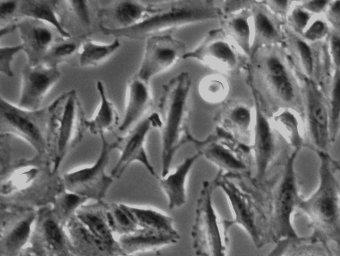
\includegraphics[width=26.5625cm, height=20cm]{pic.jpg}};
	\path (-4,0,0);
	% input
	\pic[shift={(0,0,0)}] at (0,0,0) {
		Box={
				name=input,
				caption=Input,
				xlabel= 1,
				ylabel=256,
				zlabel= \qquad 256,
				fill=\ConvColor,
				height=100,
				width=0.1,
				depth=100
			}
	};
	% conv1
	\pic[shift={(1.5,0,0)}] at (input-east) {
		RightBandedBox={
				name= conv1,
				caption=Conv1,
				xlabel={{"32",""}},
				ylabel=256,
				zlabel= \qquad 256,
				fill=\ConvColor,
				bandfill=\ConvReluColor,
				height=50,
				width=2.1,
				depth=50
			}
	};
	% MaxPool2d
	\pic[shift={(1,0,0)}] at (conv1-east) {
		RightBandedBox={
			name= MaxPool,
			xlabel={{"32",""}},
			ylabel=128,
			fill=\PoolColor,
			height=50,
			width=2.1,
			depth=50
		}
	};



	% layer1
	% conv1_1
	\pic[shift={(3,0,0)}] at (MaxPool-east) {
		RightBandedBox={
				name= conv1_1,
				xlabel={{"64",""}},
				ylabel= 128,
				fill=\ConvColor,
				bandfill=\ConvReluColor,
				height=50,
				width=2.1,
				depth=50
			}
	};
	% conv1_2
	\pic[shift={(0,0,0)}] at (conv1_1-east) {
		RightBandedBox={
				name= conv1_2,
				xlabel={{"\quad 64",""}},
				zlabel= \qquad 128,
				fill=\ConvColor,
				bandfill=\ConvReluColor,
				height=50,
				width=2.1,
				depth=50
			}
	};
	% add1_1
	\pic[shift={(1,0,0)}] at (conv1_2-east) {
		Ball={
				name=add1_1,
				fill=\SumColor,
				opacity=0.6,
				radius=2,
				logo=\(+\)
			}
	};
	% MaxPool2d_1
	\pic[shift={(1,0,0)}] at (add1_1-east) {
		RightBandedBox={
			name= MaxPool1,
			xlabel={{"64",""}},
			ylabel=64,
			fill=\PoolColor,
			height=25,
			width=4.2,
			depth=25
		}
	};

\pic[shift={(-0.2,0,0)}] at (conv1_1-west) {Box={name=env,caption=\textbf{\large{Residual Block 1}},%
		xlabel={{"","dummy"}},fill=,opacity=0.1,height=60,width={10},depth=60}};

%%%%%%%%%%%%%%%%%%%%%%%%%%%%%%%%%%
	\pic[shift={(3,0,0)}] at (MaxPool1-east) {
		RightBandedBox={
			name= conv2_1,
			xlabel={{"128",""}},
			ylabel= 64,
			fill=\ConvColor,
			bandfill=\ConvReluColor,
			height=25,
			width=4.2,
			depth=25
		}
	};
	% conv2_2
	\pic[shift={(0,0,0)}] at (conv2_1-east) {
		RightBandedBox={
			name= conv2_2,
			xlabel={{"128",""}},
			zlabel= \qquad 64,
			fill=\ConvColor,
			bandfill=\ConvReluColor,
			height=25,
			width=4.2,
			depth=25
		}
	};
	% add1_2
	\pic[shift={(1,0,0)}] at (conv2_2-east) {
		Ball={
			name=add1_2,
			fill=\SumColor,
			opacity=0.6,
			radius=2,
			logo=\(+\)
		}
	};
	% MaxPool2d_2
	\pic[shift={(1,0,0)}] at (add1_2-east) {
		RightBandedBox={
			name= MaxPool2,
			xlabel={{"64",""}},
			ylabel=32,
			fill=\PoolColor,
			height=12.5,
			width=8.4,
			depth=12.5
		}
	};

\pic[shift={(-0.4,0,0)}] at (conv2_1-west) {Box={name=env,caption=\textbf{\large{Residual Block 2}},%
		xlabel={{"","dummy"}},fill=,opacity=0.1,height=30,width={20},depth=30}};

	%%%%%%%%%%%%%%%%%%%%%%%%%%%%%%%%%%%%%%%%%%%%%%%%%
	% conv3_1
	\pic[shift={(3,0,0)}] at (MaxPool2-east) {
		RightBandedBox={
			name= conv3_1,
			xlabel={{"128",""}},
			ylabel= 16,
			fill=\ConvColor,
			bandfill=\ConvReluColor,
			height=12.5,
			width=8.4,
			depth=12.5
		}
	};
	% conv3_2
	\pic[shift={(0,0,0)}] at (conv3_1-east) {
		RightBandedBox={
		name= conv3_2,
		xlabel={{"128",""}},
		zlabel= 16,
		fill=\ConvColor,
		bandfill=\ConvReluColor,
		height=12.5,
		width=8.4,
		depth=12.5
		}
	};
	% add1_3
	\pic[shift={(1,0,0)}] at (conv3_2-east) {
		Ball={
			name=add1_3,
			fill=\SumColor,
			opacity=0.6,
			radius=2,
			logo=\(+\)
		}
	};
	% MaxPool2d_2
	\pic[shift={(1,0,0)}] at (add1_3-east) {
		RightBandedBox={
			name= MaxPool3,
			xlabel={{"128",""}},
			ylabel=16,
			fill=\PoolColor,
			height=6.25,
			width=8.4,
			depth=6.25
		}
	};

\pic[shift={(-0.6,0,0)}] at (conv3_1-west) {Box={name=env,caption=\textbf{\large{Residual Block 3}},%
		xlabel={{"","dummy"}},fill=,opacity=0.1,height=20,width={30},depth=20}};
%%%%%%%%%%%%%%%%%%%%%%%%%%%%%%%%%%%%%%%%%

	% fullconnection
	\pic[shift={(2,0,0)}] at (MaxPool3-east) {
		RightBandedBox={
				name=fc1,
				caption=\makebox[0pt]{
					 \shortstack[c]{\\ FC1}},
				xlabel={{"1",""}},
				zlabel=\qquad 1024,
				fill=\FlattenColor,
				height=2,
				width=2,
				depth=100
			}
	};
	\pic[shift={(2,0,0)}] at (fc1-east) {
		RightBandedBox={
				name=fc2,
				caption=\makebox[0pt]{
					 \shortstack[c]{\\ FC2 \\Sigmoid}},
				xlabel={{"1",""}},
				zlabel=\qquad 1,
				fill=\FcColor,
				bandfill=\FcSigmoidColor,
				height=2,
				width=2,
				depth=2
			}
	};

	% connections
	\draw [connection]  		(input-east)			-- 	node {\midarrow} 	(conv1-west);
	\draw [connection]  		(conv1-east)			-- 	node {\midarrow} 	(MaxPool-west);
	\draw [connection] (MaxPool-east) -- node {\midarrow} (conv1_1-west);


	% connections shortcut
	% conv1 to add1_1
	\path (MaxPool-east) -- (conv1_1-west) coordinate[pos=0.5] (pool_conv1_1);
	\path (pool_conv1_1) ++ (0,5,0) coordinate (pool_conv1_1_above);
	\path (add1_1-north) ++ (0,5,0) coordinate (add1_1-north-above);
	
	\draw [connection] (pool_conv1_1) -- node {\midarrow} (pool_conv1_1_above|-add1_1-north-above) -- node {\midarrow} (add1_1-north-above) -- node {\midarrow} (add1_1-north);
	\draw [connection] (conv1_2-east) -- (add1_1-west);
	\draw [connection] (add1_1-east) -- node {\midarrow} (MaxPool1-west);
	\draw [connection] (MaxPool1-east) -- node {\midarrow} (conv2_1-west);
	
	%
	\path (MaxPool1-east) -- (conv2_1-west) coordinate[pos=0.65] (add_conv_1);
	\path (add_conv_1) ++ (0,5,0) coordinate (add_conv_1-above);
	\path (add1_2-north) ++ (0,5,0) coordinate (add1_2-north-above);
	\draw [connection] (add_conv_1) -- node {\midarrow} (add_conv_1-above|-add1_2-north-above) -- node {\midarrow} (add1_2-north-above) -- node {\midarrow} (add1_2-north);
	\draw [connection] (conv2_2-east) -- (add1_2-west);
	\draw [connection] (add1_2-east) -- node {\midarrow} (MaxPool2-west);
	\draw [connection] (MaxPool2-east) -- node {\midarrow} (conv3_1-west);

	%%%%%%%%%%%%%%
	\path (MaxPool2-east) -- (conv3_1-west) coordinate[pos=0.75] (add_conv_2);
	\path (add_conv_2) ++ (0,5,0) coordinate (add_conv_2-above);
	\path (add1_3-north) ++ (0,5,0) coordinate (add1_3-north-above);
	\draw [connection] (add_conv_2) -- node {\midarrow} (add_conv_2-above|-add1_3-north-above) -- node {\midarrow} (add1_3-north-above) -- node {\midarrow} (add1_3-north);
	\draw [connection] (conv3_2-east) -- (add1_3-west);
	\draw [connection] (add1_3-east) -- node {\midarrow} (MaxPool3-west);

	% pool & fullconnection
	\draw	[densely dashed]  (MaxPool3-nearnortheast)    	--  									(fc1-nearnorthwest);
	\draw	[densely dashed]  (MaxPool3-nearsoutheast)    	--  									(fc1-nearsouthwest);
	\draw	[densely dashed]  (MaxPool3-farnortheast)    	--  									(fc1-farnorthwest);
	\draw	[densely dashed]  (MaxPool3-farsoutheast)    	--  									(fc1-farsouthwest);
	%
	\draw	[densely dashed]  (fc1-nearnortheast)    	--  									(fc2-nearnorthwest);
	\draw	[densely dashed]  (fc1-nearsoutheast)    	--  									(fc2-nearsouthwest);
	\draw	[densely dashed]  (fc1-farnortheast)    	--  									(fc2-farnorthwest);
	\draw	[densely dashed]  (fc1-farsoutheast)    	--  									(fc2-farsouthwest);
	%%%%%%%%%%%%%%%%%%%%%%%%%%%%%%%%%%%%%%%%%%%%%%%%%%%%%%%%%%%%%%%%%%%%%%%%%%%%%%%%%%%%%%%
\end{tikzpicture}
\end{document}